\documentclass{article}
\usepackage[utf8]{inputenc}

\title{Demostración de la NP-Completitud del problema CLIQUE}
\author{ Alejandro León Fernández \\
    Javier Esteban Pérez Rivas \\
    Sara Revilla Báez}
\date{16 de enero de 2019}

\usepackage{natbib}
\usepackage{graphicx}
\usepackage{booktabs} % Allows the use of \toprule, \midrule and \bottomrule in tables
\usepackage{amsmath}

% Spanish
\usepackage[spanish]{babel}
\usepackage[utf8]{inputenc}

\begin{document}

\maketitle

\newpage

\tableofcontents

\newpage

\section{Introducción}

\subsection{¿Qué es un clique?}
El término se usó por primera vez en un trabajo Luce \& Perry (1949) en referencia a los grupos de personas que se conocen entre todas ellas. \\

De manera informal, un \textit{\textbf{clique}} es un subconjunto de vértices de un grafo no dirigido, tal que cada par de vértices sea adyacente. Es decir, que su subgrafo inducido es completo. \\

\begin{figure}[h!]
\centering
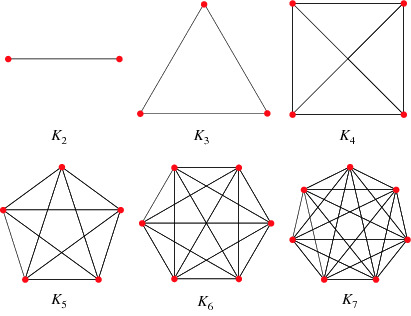
\includegraphics[width=0.8\linewidth]{img/complete_graphs.jpg}
\caption{Distribución de cliques en función de su tamaño}
\end{figure}
%---------------------------------------------------
\subsection{Descripción del problema}
Dado un grafo $G = (V, E)$ y un entero positivo $k$:\\

\centerline{¿Existe un \textit{\textbf{k-clique}} en $G$?}

Es decir, que si existe un conjunto de vertices $V' \subseteq V$ tal que, 
$$ |V'| \geq k $$
$$ \forall u, v \in S \implies \exists (u, v) \in E $$
%----------------------------------------------------
\section{Demostración de NP-Completitud}
Para poder demostrar que un problema es  \textit{\textbf{NP-Completo}}, debemos probar que:

\begin{itemize}
    \item El problema pertenece a la clase \textit{\textbf{NP}}.
    \item {Existe una transformación de cualquier problema de la clase \textit{\textbf{NP}}  a dicho problema o que, alternativamente, existe una transformación de un problema \textit{\textbf{NP-Completo}} a este problema.
\end{itemize}

\subsection{CLIQUE pertenece a NP}
\textit{“Si encontramos un algoritmo no determinista que decida si para un grafo G = (V, E) existe un clique de tamaño mayor o igual que k, entonces podemos afirmar que el problema de CLIQUE $\in$ NP”}\\

Para ello, bastaría con probar con todos los $V' \subseteq V$ tal que $\vert V' \vert \geq k$ y ver si existe un clique de tamaño  mayor o igual a k. Esta comprobación se puede realizar en tiempo polinomial mirando que $(u,v) \in E$ para cada $u, v \in S$, lo cual tiene complejidad $O(n^2)$.
%-----------------------------------------------------

\subsection{Transformación de un problema NP-Completo a CLIQUE}
Existe una secuencia de transformaciones que permiten demostrar que el CLIQUE es reducible al SAT de manera prácticamente trivial (comparándolo con el \textit{\textbf{Vertex Cover}}). Sin embargo, vamos a plantear una transformación directa del 3-SAT al CLIQUE

\begin{figure}[h!]
\centering
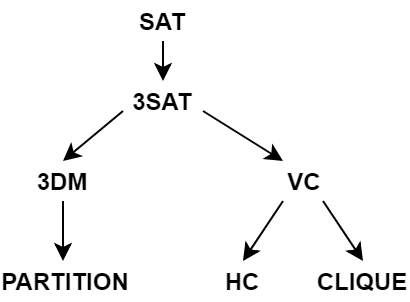
\includegraphics[width=0.8\linewidth]{img/problem-diagram.png}
\caption{Diagrama de la secuencia de transformaciones de los 6 problemas básicos}
\end{figure}
%-----------------------------------------------------

\subsection{Descripción del Problema 3-SAT}
Dada una colección $C = \{c_{1}, c_{2}, ..., c_{m}\}$ de cláusulas con un conjunto $X = \{x_{1}, x_{2}, ..., x_{n}\}$ de variables, tal que $\vert c_{i} \vert$ = 3 para $1 \geq \textit{i} \geq m$\\

\centerline{¿Existe alguna asignación de verdad para $X$ que satisfaga todas las cláusulas en $C$?}
%----------------------------------------------------

\subsection{Transformación del 3-SAT al CLIQUE}
 Sea $\phi$ una instancia de 3-SAT tal como hemos descrito, y cada cláusula $c_{i} = \{z_{i1}, z_{i2}, ..., z_{it}\}$ (con $t = 3$), necesitamos construir una instancia del CLIQUE (un grafo), que sea positiva si, y sólo si, $\phi$ también es positiva.\\
 
  Construimos un grafo $G = (V,E)$ de la siguiente forma:
\begin{enumerate}
    \item En primer lugar añadimos $t$ nodos por cada cláusula. Este paso se hace en tiempo $O(t \cdot m)$ que es $O(m)$,  ya que t es constante ($t = 3$).
    \item Para cada par de nodos $v_{ab},v_{cd}$ en $G$, añadimos la arista $(v_{ab},v_{cd})$ si, y sólo si:
    \begin{itemize}
        \item $a \neq c$
        \item $z_{ab} \neq \bar{z}_{cd}$
    \end{itemize}
\end{enumerate}\\

\centerline{\textbf{ $\phi$ es satisfactible si y solo si $G$ tiene un clique de tamaño $k \geq m$.}}
%---------------------------------------------------

\subsection{Demostración}
Si $\phi$ es satisfactible, elegimos un literal satisfecho de cada cláusula obteniendo $\{z_{1}^{*}, z_{2}^{*}, ..., z_{m}^{*}\}$, siendo $\{v_{1}, v_{2}, ..., v_{m}\}$ los nodos correspondientes en $G$. Dicho conjunto de nodos forma un \textit{\textbf{m-clique}}, pues estarán conectados ya que:
\begin{itemize}
    \item Hemos escogido los literales de diferentes cláusulas
    \item No puede haber contradicciones entre los literales escogidos porque $\phi$ es satisfactible
\end{itemize}

De manera inversa, supongamos que $G$ tiene un clique de tamaño $m = k$ o mayor. Sea $\{v_{1}, v_{2}, ..., v_{q}\}$ un clique en $G$ de tamaño $q \geq m$. Entonces los $m$ primeros nodos $\{v_{1}, ..., v_{m}\}$ también forman un clique en $G$.
\begin{itemize}
    \item Dado que no hay aristas conectando nodos que vengan de la misma cláusula, cada uno de los nodos corresponde a un literal de una cláusula.
    \item Además, no hay nodos que vengan de literales opuestos conectados debido a la construcción realizada
\end{itemize}
Así, para satisfacer $\phi$ basta con satisfacer $\{z_{1}, ..., z_{m}\}$ y asignar las variables restantes de forma arbitraria.
%---------------------------------------------------
\section{Ejemplo}
Sea $\phi$ una instancia de 3-SAT, con variables $x_{i}$, para $i$ en $1 \leq i \leq 3$, se obtiene el siguiente grafo aplicando la reducción comentada anteriormente. 

$$\phi = (x_{1}\lor \bar{x}_{2} \lor \bar{x}_{3}) \land (\bar{x}_{1} \lor x_{2} \lor x_{3}) \land (x_{1} \lor x_{2} \lor x_{3})$$

\begin{figure}[h!]
\centering
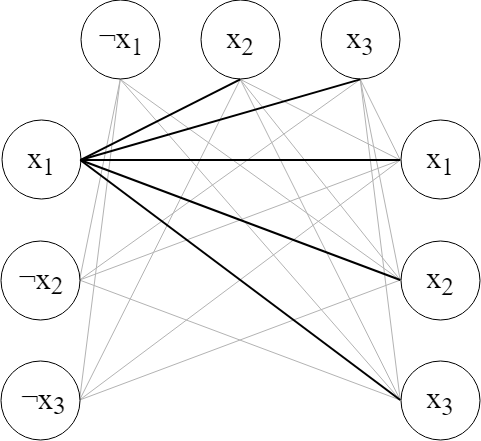
\includegraphics[width=0.8\linewidth]{img/Grafo_Ejemplo_Clique.png}
\caption{Grafo resultante de $\phi$}
\end{figure}

En la figura 3, se puede observar como el grafo tiene 9 nodos, ya que $\phi$ tiene 3 cláusulas, y que no hay aristas entre nodos de la misma cláusula. Además, las aristas marcadas en negro corresponden con la uniones que habría entre el nodo ${x}_{1}$ de la primera cláusula, con el resto de nodos. Se aprecia que entre ${x}_{1}$ y $\bar{x}_{1}$ no se crea arista, pues se generarían contradicciones.\\

Elegimos una variable, $z_{i}$, dentro de cada cláusula y suponemos que es verdadera. Cada una se corresponde con un nodo dentro del grafo. $\phi$ se podrá satisfacer si, y sólo si, existe un \textbf{clique} para los nodos elegidos. Para este ejemplo, elegiremos $x_{1}$ como variable positiva de la primera cláusula,  $x_{2}$, para la segunda, y $x_{3}$, para la tercera.

\begin{figure}[h!]
\centering
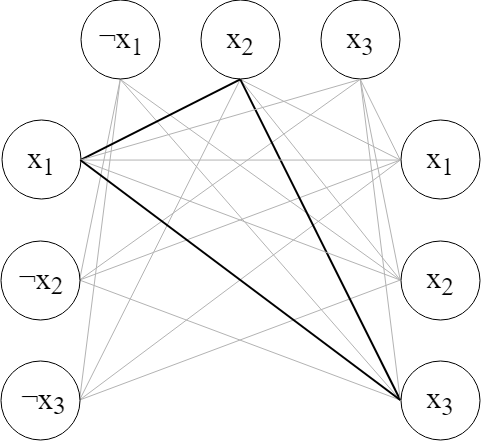
\includegraphics[width=0.8\linewidth]{img/Grafo_Seleccion_Clique.png}
\caption{Clique obtenido con los nodos establecidos}
\end{figure}

Al elegir estos nodos, como se puede ver en la figura 4, existe un \textit{\textbf{clique}} que conecta los tres nodos, por lo que, de este modo,  $\phi$ se podría satisfacer.

\footnotesize{
    \begin{thebibliography}{99}
        \bibitem{GareyJohnson}
            Michael Garey, David S. Johnson.
        \newblock {\em Computers and Intractability: A Guide to the Theory of NP-Completeness}.
        \newblock W. H. Freeman and Company, 1979.
        
        \bibitem{Mouatadid}
            Lalla Mouatadid.
        \newblock {\em Introduction to Complexity Theory: CLIQUE is NP-complete}.
        \newblock CSC 373 - Algorithm Design, Analysis, and Complexity, Summer 2014.
    \end{thebibliography}
}
\end{document}
